\documentclass[a4paper, 12pt]{exam}

\usepackage[onehalfspacing]{setspace}
\usepackage{graphicx}
\usepackage{amsmath,amsfonts,amsthm,amssymb,mathtools}
\usepackage{nameref}
\usepackage{hyperref}
\usepackage{xcolor}
\usepackage{color,soul}
\usepackage{gensymb}
\usepackage[]{booktabs}
\usepackage[utf8]{inputenc}
\usepackage{array}
\usepackage{setspace}
\usepackage{verbatim} %for multiline comments https://tex.stackexchange.com/questions/44282/multiline-comment
\usepackage{xhfill}
\usepackage{enumitem}
\usepackage{varwidth}
\usepackage{multicol, array}
\usepackage{etoolbox}
\usepackage{multicol}
\usepackage[most,many,breakable]{tcolorbox}
\usepackage{mathtools}
\usepackage{background} %Package for adding a watermark
\usepackage{tikz-cd}
\usepackage{pgfplots} 
\pgfplotsset{compat=newest}
\usepgfplotslibrary{patchplots}
\usepackage{anyfontsize}
\usepackage{sectsty}
\usepackage[space]{grffile} %To allow for spaces in the path for the watermark
\usepackage{amsmath}
\usepackage{geometry} %lets us set the margins of the page
\usepackage{comment} %Allows for multi-line comments (\ifx \fi)
\usepackage{import} %lets us perform multi-file compilation
\usepackage{pdfpages} %allows for the inclusion of external multi-page PDF documents
\usepackage{algpseudocode} %lets you write algorithms (probably won't be used but i'm including it anyways) https://www.overleaf.com/learn/latex/Algorithms
\usepackage{bookmark}
\usepackage{theorem}

\usepackage{caption}


\usetikzlibrary{arrows, decorations.markings}
\usepackage{fontawesome}

\usetikzlibrary{hobby,backgrounds,positioning}
\usepackage{tikzsymbols}
\tikzsymbolsset{%
  after-symbol={},
}


\geometry{left=0.8in,top=0.5in, right = 0.8in}

\newcommand{\cuspac}{\hspace*{1cm}}

\backgroundsetup{contents=\includegraphics{Anant_Logo.png}, opacity=0.1, angle=0, scale=1.5}

\begin{document}
	\title{Anant 24-25 Recruitment Test}
	\author{Attitude Determination and Controls Subsystem (ADCS)}
	\date{January 12th, 2024}
	\maketitle
	
	\section*{Instructions}
	All general instructions are provided in the Google Classroom. Make sure you refer to them for submission details. Failure to adhere to the given rules may result in disqualification. 
	\begin{enumerate}[]
		\item This paper relies more on comprehension and general aptitude than it does in depth knowledge of the subject. You are encouraged to use the internet to solve this paper.
		\item Any changes to the paper will be posted in Google Classroom and an updated file will be shared. Please keep an eye out.
	\end{enumerate} 
	
	\bigskip

	\begin{enumerate}[label = \textbf{Rule \arabic* }:, leftmargin=5em]
		\item A student must prioritize developing an understanding of the topics being tested and demonstrating general aptitude, as evaluated during the subsequent interview where their solutions will be the main topic of discussion.
		
		\item A student must not collaborate with peers unless such collaboration is necessary to better achieve the goals outlined in Rule 1.
		
		\item A student must prioritize their physical and mental well-being, avoiding undue stress, all-nighters, or harmful study practices, unless doing so would conflict with Rules 1 or 2.
		
			\end{enumerate}
		
If you have any questions regarding the content of the paper, feel free to reach out to any of the undersigned for help. \\

Contact Details:
		\begin{enumerate}
			\item Aaditya Thakkar - +91 81282 17114
			\item Nikhil Mathew - +91 97400 44411
			\item Pranav Chandra - +91 90807 96426
			\item Pramit Pal - +91 99026 97222
		\end{enumerate}

	\begin{center}
		\textbf{All the best!}
	\end{center}
		
	\pagebreak
	
	\newgeometry{left=0.75in,top=1in, right = 0.75in}
	

\section*{Question 1: Coordinate transformations and orbital mechanics}

\noindent $(a)$ Using the provided Earth-Centered Earth-Fixed (ECEF) coordinates of $(3182.655, 2000.94, 5135.159) \, \text{km}$, calculate the corresponding latitude, longitude, and altitude of the point on Earth's surface. Additionally, determine the physical location (name of the place) on Earth corresponding to these coordinates.

\bigskip

\noindent $(b)$ Convert the position from the Earth-Centered Earth-Fixed (ECEF) frame to the Earth-Centered Inertial (ECI) frame for today's date and time. Assume that the ECEF and ECI frames align perfectly at 1200 GMT daily.

\bigskip

\noindent $(c)$ For the date January 2, 1920, at 1420 VLAT (UTC+10:00), calculate the Earth's position in its orbit around the Sun using celestial mechanics. Parameterize the Earth's position in an elliptical orbit with:
\begin{itemize}
    \item The origin at the center of the Sun.
    \item The \( z \)-axis perpendicular to the orbital plane, pointing north.
    \item The \( x \)-axis pointing toward the Sun at perihelion.
\end{itemize}
Re-convert the ECEF coordinates to the Earth-Centered Inertial (ECI) frame for this historical date and input the converted coordinates.

	
	\pagebreak

\section*{Question 2: Orbital mechanics and gravitational anomalies}

\noindent $(a)$ Calculate the $\Delta V$ required for an orbit transfer maneuver as depicted in the image below to move a spacecraft from a circular orbit of 200 km altitude to a circular orbit of 2000 km altitude. Assume a central body with a radius of 6371 km and a standard gravitational parameter $\mu = 3.986 \times 10^{14} \, \text{m}^3/\text{s}^2$.

	\begin{center}
	\begin{tikzpicture}[ scale=1.250,
    >=triangle 45,
    mydeco/.style = {
        decoration = {
            markings, 
            mark = at position #1 with {
                \node[scale=1.2, rotate=\pgfdecoratedangle+140] {\faRocket};
            }
        }
    }
]
                      
         \draw (-1,-0.165) node[rotate=180, color=orange, scale = 1.5] {\Fire};
    \draw (-1.05,0) node [anchor = east, scale = 0.75, color=orange]  {$1^{st} \ Burn \ \ $};
    \draw (2.5,0.05) node[rotate=0, color=orange, scale = 1.5] {\Fire};
    \draw (2.5,0) node [anchor = east, scale = 0.75, color=orange]  {$2^{nd} \ Burn \ \ $};                 
                      
    \filldraw[top color = blue!75!green, bottom color = blue!60, opacity = .75] (0,0) circle (.5cm);
    
    \draw[postaction = {mydeco=-0.2416 ,decorate}, 
          postaction = {mydeco=-0.58333 ,decorate},
          postaction = {mydeco=-0.0075 ,decorate}]
          (0,0) circle (2.5cm);

    \draw[postaction = {mydeco=-0.375 ,decorate}, 
          postaction = {mydeco=-0.875 ,decorate}] (0,0) circle (1cm);
    \draw (0.65,-1.2) node [anchor = east, scale = 0.8]  {Initial Orbit};
    

    \draw[postaction = {mydeco=0.5 ,decorate, color=black}, 
          postaction = {mydeco=0.9975 ,decorate, color=black}, color = orange, thick] (0:2.5) arc (0:180:1.75cm and 1.3cm);
     \draw (0.65,2.7) node [anchor = east, scale = 0.8]  {Final Orbit};
    



	\end{tikzpicture}
	\end{center}

\bigskip

\noindent $(b)$ Consider a two-stage transfer where the spacecraft first transitions to an intermediate high-altitude orbit before reaching the final circular orbit at 2000 km altitude. Calculate the total $\Delta V$ for this three-burn maneuver. Compare the result with the $\Delta V$ from part $(a)$. Explain the circumstances under which this method might be preferred over the maneuver in part $(a)$.

	\begin{center}
	\begin{tikzpicture}[ scale=1.50,
    >=triangle 45,
    mydeco/.style = {
        decoration = {
            markings, 
            mark = at position #1 with {
                \node[scale=1.2, rotate=\pgfdecoratedangle+140] {\faRocket};
            }
        }
    }
]
                      
        \draw (-1,-0.15) node[rotate=180, color=orange, scale = 1.5] {\Fire};
    \draw (-1,0) node [anchor = east, scale = 0.75, color=orange]  {$1^{st} \ Burn \ \ $};
    \draw (5,0.15) node[rotate=0, color=orange, scale = 1.5] {\Fire};
    \draw (5,0) node [anchor = east, scale = 0.75, color=orange]  {$2^{nd} \ Burn \ \ $};
    \draw (-2.5,-0.165) node[rotate=180, color=orange, scale = 1.5] {\Fire};
    \draw (-2.5,0) node [anchor = east, scale = 0.75, color=orange]  {$3^{rd} \ Burn \ \ $};
    
    \filldraw[top color = blue!75!green, bottom color = blue!60, opacity = .75] (0,0) circle (.5cm);
    
    \draw[ color = teal] (0:5) arc (0:-180:3.75cm and 3.2cm);
    %\draw[ color = teal, dashed] (0:5) arc (0:180:3.75cm and 3.2cm);
    \draw (2,-3.35) node [anchor = east, scale = 0.8, text=teal]  {Transfer Orbit 2};
    
        \draw[ 
          postaction = {mydeco=0.9975 ,decorate, color=black},postaction = {mydeco=0 ,decorate, color=black}, color = orange] (0:5) arc (0:180:3cm and 1.7cm);
         % \draw[color = orange, dashed] (0:5) arc (0:-180:3cm and 1.7cm);
          \draw (3.5,1.8) node [anchor = east, scale = 0.8, text=orange]  {Transfer Orbit 1};
 
    
    \draw[postaction = {mydeco=-0.2416 ,decorate}, 
          postaction = {mydeco=-0.68333 ,decorate},
          postaction = {mydeco=-0.5 ,decorate},]
          (0,0) circle (2.5cm);

    \draw[postaction = {mydeco=-0.15 ,decorate}, 
          postaction = {mydeco=-0.75 ,decorate}] (0,0) circle (1cm);
    \draw (1.65,-1) node [anchor = east, scale = 0.8]  {Initial Orbit};
    


          
          
          
     \draw (1.65,2.55) node [anchor = east, scale = 0.8]  {Final Orbit};
    

    


	\end{tikzpicture}
\end{center}



\bigskip

\noindent $(c)$ In an alternate universe, the gravitational force is given by $F = G \frac{m_1 m_2}{r^3}$. Derive the resulting orbital characteristics under this new force law. Specifically:
\begin{itemize}
    \item Determine the shape and stability of the orbits.
    \item Calculate how the maneuvers required for orbital transfers would change compared to the standard $r^{-2}$ gravitational law.
\end{itemize}

\bigskip

\noindent \textbf{Note:} Assume standard units for mass, distance, and time throughout. Provide all derivations and necessary equations in your solutions.
	
	\pagebreak
	

\section*{Question 3: Positioning, velocity, and orientation in space}

\noindent $(a)$ A spacecraft in deep space is equipped with a GPS-like system that communicates with satellites. The coordinates of three satellites are provided:
\[
\begin{aligned}
\text{Satellite A: } (-3141, -5926, 5358) \, \text{km} \\
\text{Satellite B: } (-9793, 2384, -6264) \, \text{km} \\
\text{Satellite C: } (3383, -2795, -0288) \, \text{km}
\end{aligned}
\]
The fourth satellite's coordinates are unknown but follow the symmetry rule: \(x = y = z\). The signal travel times to the spacecraft from the four satellites are as follows:
\[
t_A = 23.90987365 \, \text{ms}, \quad
t_B = 51.57336220 \, \text{ms}, \quad
t_C = 21.79227717 \, \text{ms}, \quad
t_D = 14.96656189 \, \text{ms}.
\]
Using this data, determine:
\begin{itemize}
    \item $(i)$ The spacecraft's position in Cartesian coordinates.
    \item $(ii)$ The coordinates of the fourth satellite.
\end{itemize}

\bigskip

\noindent $(b)$ After a system malfunction, the spacecraft can only receive signals from three satellites. The following ping times are recorded for two separate instances at timestamps \(t_1 = 0 \, \text{s}\) and \(t_2 = 5000 \, \text{s}\):
\[
\begin{aligned}
A_1 &= 28.21941442 \, \text{ms}, & A_2 &= 32.56521822 \, \text{ms}, \\
B_1 &= 37.40539321 \, \text{ms}, & B_2 &= 37.48077648 \, \text{ms}, \\
C_1 &= 21.88477974 \, \text{ms}, & C_2 &= 35.47581482 \, \text{ms}.
\end{aligned}
\]
Using this data, calculate the spacecraft's velocity vector.

\bigskip

\noindent $(c)$ The spacecraft's GPS system is damaged, leaving only a sun sensor, a magnetic field sensor, and a radio transmitter functional. Determine how to use these sensors to calculate the spacecraft's orientation relative to Earth. Include a sketch in your solution showing how the sensors' data can provide the required orientation information.
	
\pagebreak
\section*{Question 4: Position estimation and prediction}

\noindent $(a)$ A target object is observed at various positions over time. The first \(n\) observed positions are:
\[
(x_1, y_1), (x_2, y_2), \dots, (x_n, y_n).
\]
Using this data, estimate the target object's true position. Provide a clear calculation method and explanation.

\bigskip

\noindent $(b)$ Derive a formula that dynamically updates the estimated position of the target using the \(k\)-th estimation and the \((k+1)\)-th measurement. Explain how the formula refines the estimate with each new measurement.

\bigskip

\noindent $(c)$ Using the provided measurements below, estimate the true position of the target and calculate its distance from the observer:
\[
\begin{aligned}
\{ 
&(-4.135, 2.81), \quad (-4.859, -1.178), \quad (-3.52, 3.551), \quad (-4.543, 2.088), \quad  (-4.185, 2.736), \\
&(-4.993, 0.269), \quad (-4.455, 2.27), \quad (-1.566, 4.748), \quad (-4.843, -1.243), \quad (-4.848, 1.222)
\}.
\end{aligned}
\]

\bigskip

\noindent $(d)$ The target object is observed to drift with an angular velocity of $\omega = \frac{2\pi}{14} \, \text{rad/s}$. Using the first \(n\) measurements, estimate the target’s position at a future time \(t = t_k\). Show your calculations clearly.

\bigskip

\noindent $(e)$ Using the following measurements over the first 5 seconds:
\[
\begin{aligned}
\{ 
&(-4.349, 2.468), \quad (-4.789, 1.438), \quad (-4.898, 1.003), \quad (-4.741, 1.588), \quad (-4.92, 0.893), \\
&(-4.92, -0.893), \quad (-3.471, -3.598), \quad (1.373, -4.808), \quad (2.428, -4.371), \quad (4.315, -2.526)
\},
\end{aligned}
\]
predict the target's position at \(t = 5.5 \, \text{s}\) based on the observed drift and angular velocity. Provide your prediction and explain your approach.

\bigskip

\end{document}